\documentclass{ctexart}
\PassOptionsToPackage{numbers,compress}{natbib}
% Common packages
\usepackage[utf8]{inputenc} % allow utf-8 input
\usepackage[T1]{fontenc}    % use 8-bit T1 fonts
\usepackage{microtype}
\usepackage{times}
\usepackage{graphicx}
\usepackage{amsmath,amssymb,mathbbol}
% \usepackage{algorithmic}
% \usepackage[linesnumbered,ruled,vlined]{algorithm2e}
\usepackage{acronym}
\usepackage{enumitem}
\usepackage[pagebackref=true,breaklinks=true,colorlinks]{hyperref}
\usepackage{balance}
\usepackage{xspace}
\usepackage{setspace}
\usepackage[skip=3pt,font=small]{subcaption}
\usepackage[skip=3pt,font=small]{caption}
\usepackage[dvipsnames]{xcolor}
\usepackage[capitalise]{cleveref}
\usepackage{booktabs,tabularx,colortbl,multirow,array,makecell}
\usepackage{indentfirst} 
% \usepackage{overpic,wrapfig}

\usepackage{fancyhdr}
\hypersetup{pdfencoding=auto,colorlinks=true,allcolors=black}
\renewcommand{\headrulewidth}{0.5pt}
\renewcommand{\footrulewidth}{0pt}
\fancyhf{}
\fancyhead[C]{}
\fancyhead[C]{}
\fancyfoot[C]{\thepage}

% Handy shorthand
\makeatletter
\DeclareRobustCommand\onedot{\futurelet\@let@token\@onedot}
\def\@onedot{\ifx\@let@token.\else.\null\fi\xspace}
\def\eg{\emph{e.g}\onedot} 
\def\Eg{\emph{E.g}\onedot}
\def\ie{\emph{i.e}\onedot} 
\def\Ie{\emph{I.e}\onedot}
\def\cf{\emph{c.f}\onedot} 
\def\Cf{\emph{C.f}\onedot}
\def\etc{\emph{etc}\onedot} 
\def\vs{\emph{vs}\onedot}
\def\wrt{w.r.t\onedot} 
\def\dof{d.o.f\onedot}
\def\etal{\emph{et al}\onedot}
\makeatother

\definecolor{gray}{gray}{0.9}

% Handy math ops
\DeclareMathOperator*{\argmax}{arg\,max}
\DeclareMathOperator*{\argmin}{arg\,min}
\newcommand{\norm}[1]{\left\Vert #1 \right\Vert}

% % Spacing
\frenchspacing
% \medmuskip=2mu   % reduce spacing around binary operators
% \thickmuskip=3mu % reduce spacing around relational operators
% \setlength{\abovedisplayskip}{3pt}
% \setlength{\belowdisplayskip}{3pt}
% \setlength{\abovecaptionskip}{3pt}
% \setlength{\belowcaptionskip}{3pt}
\setlength\floatsep{0.5\baselineskip plus 3pt minus 2pt}
\setlength\textfloatsep{0.5\baselineskip plus 3pt minus 2pt}
\setlength\dbltextfloatsep{0.5\baselineskip plus 3pt minus 2pt}
\setlength\intextsep{0.5\baselineskip plus 3pt minus 2pt}

\makeatletter
\renewcommand{\paragraph}{%
  \@startsection{paragraph}{4}%
  {\z@}{0ex \@plus 0ex \@minus 0ex}{-1em}%
  {\hskip\parindent\normalfont\normalsize\bfseries}%
}
\makeatother

% Graphics path
\graphicspath{{figures/}}

% Clever references
\crefname{algorithm}{Alg.}{Algs.}
\Crefname{algorithm}{Algorithm}{Algorithms}
\crefname{section}{Sec.}{Secs.}
\Crefname{section}{Section}{Sections}
\crefname{table}{Tab.}{Tabs.}
\Crefname{table}{Table}{Tables}
\crefname{figure}{Fig.}{Fig.}
\Crefname{figure}{Figure}{Figure}

% Acronym
\acrodef{pku}[PKU]{Peking University}
\usepackage[final]{template22}
\setlength{\parindent}{2em}

\title{Lab3  MLP reconstruction}
\author{王想 2100013146}
\date{}
\begin{document}
\maketitle

\section{Implementation}
\subsection{Model Structure}
我用MLP拟合一个从坐标到SDF值的函数,
进而得到物体的隐式表达。
Lab中我采用的MLP模型整体结构有6层,
中间的4层隐藏线性层的维度均设置为512维,
除了最后一层之外,其他5层后面都接入一个激活函数Softplus。
Note:一个MLP只对应一个输入的点云的隐式表达。
经过实验,我发现只需要4层隐藏层就足以获得足够好的效果,
所以我并未采用更深的网络。
MLP网络拟合的函数可以用公式表达为:
$$f:\mathbb{R}^3 \rightarrow \mathbb{R} $$
$$f(pos ,\theta)=sdf(pos) $$
$\theta$为MLP网络的模型参数,$pos$为点的坐标,$sdf(pos)$表示位置$pos$上的SDF值。
$$ $$

\subsection{Loss Function}
损失函数我采用论文Implicit Geometric Regularization for Learning Shapes(IGR)
中的损失函数,定义如下:
\begin{figure}[htbp]
    \centering
    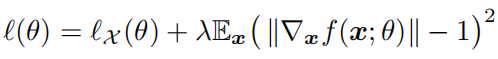
\includegraphics[width=0.4\linewidth]{figures/loss.png}
\end{figure}
\begin{figure}[htbp]
    \centering
    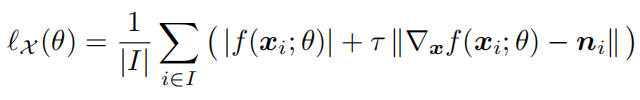
\includegraphics[width=0.5\linewidth]{figures/loss1.png}
\end{figure}

以上两式中,函数$f(\cdot ,\theta)$为MLP模型;$\chi$ 为输入的点云,
$I$为输入的点云中的点的索引构成的集合;
$x$为点的坐标,$n_i$为点的法向;
$\mathbb{E}(\cdot) $表示数学期望;
$\lambda, \tau $均为超参数,
这两个参数我遵循原论文的设置,$\lambda=0.1, \tau=1.0 $。

但是在具体实现时原论文还加上了一项$Latent Loss$用于将MLP网络泛化到所有点云
(原论文作者希望训练好一个MLP就能运用到很多不同的点云上),
而在我的实现中我去掉了这一项,这是因为本次Lab的目标是针对这一个特定的点云进行重建,
在这个场景下拟合的越接近越好,
所以并不需要加上促使模型泛化的$Latent Loss$。
最后得出的效果证明我这样的舍弃是没问题的。
$$$$

\subsection{Decoder}
在MLP模型训练好后,得到的就是这个物体的隐式表达。
从隐式表达解码出显示表达流程如下,
对给定的分辨率$r$,先生成立方体网格,
即$r^3$个对应的网格采样点,
然后将这些点的坐标输入MLP网络得到对应位置上的SDF值,
最后利用MarchingCube算法得到显示表达,即Mesh表达。
$$$$



\section{Results}
在默认参数设置下,用$RTX\ 3050\ Ti$训练需要4min20s左右,解码需要10s左右。
以下是在默认参数设置下得到的结果,可以看到重建出来的网格质量较高。
\begin{figure}[htbp]
    \centering
    \begin{subfigure}[htbp]{0.24\linewidth}
        \centering
        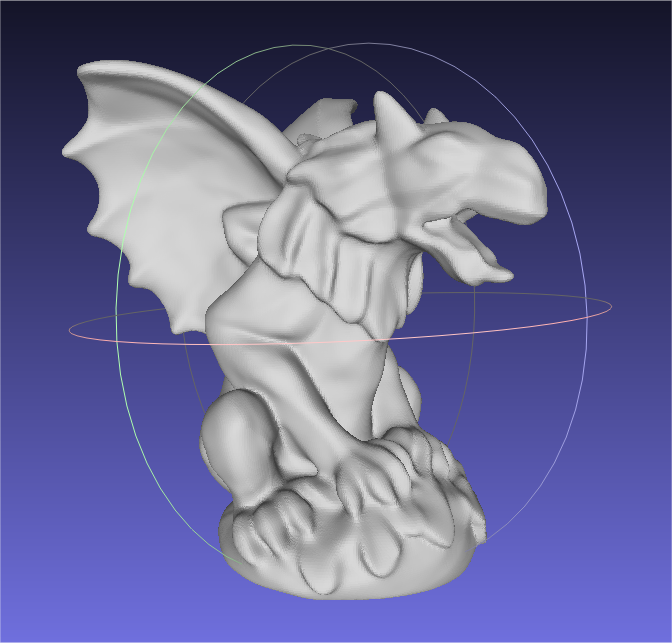
\includegraphics[width=0.9\linewidth]{figures/1.png}
    \end{subfigure}
    \begin{subfigure}[htbp]{0.24\linewidth}
        \centering
        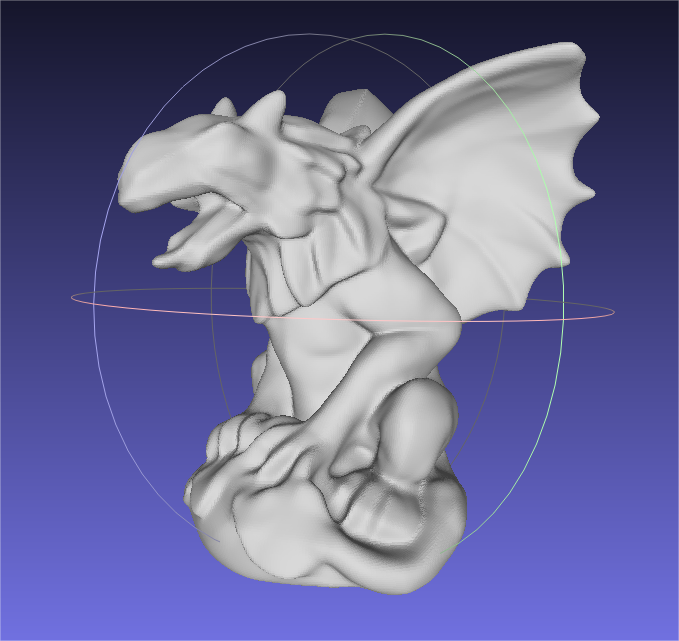
\includegraphics[width=0.9\linewidth]{figures/2.png}
    \end{subfigure}
    \begin{subfigure}[htbp]{0.24\linewidth}
        \centering
        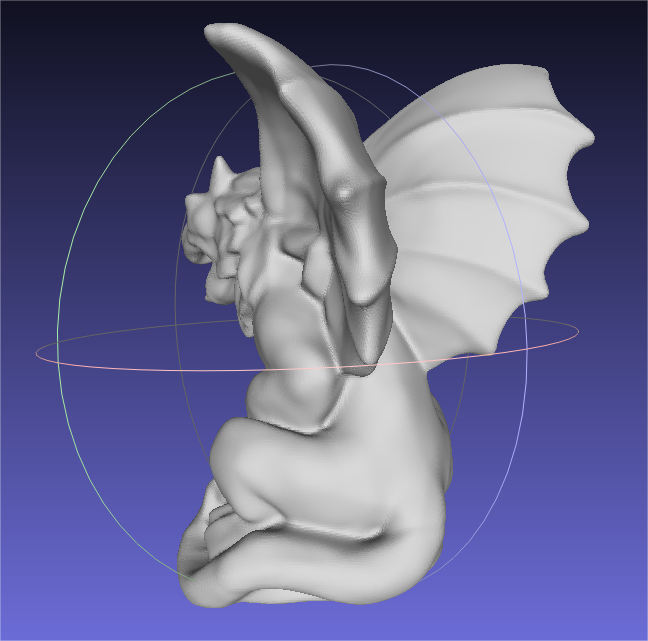
\includegraphics[width=0.9\linewidth]{figures/3.png}
    \end{subfigure}
    \begin{subfigure}[htbp]{0.24\linewidth}
        \centering
        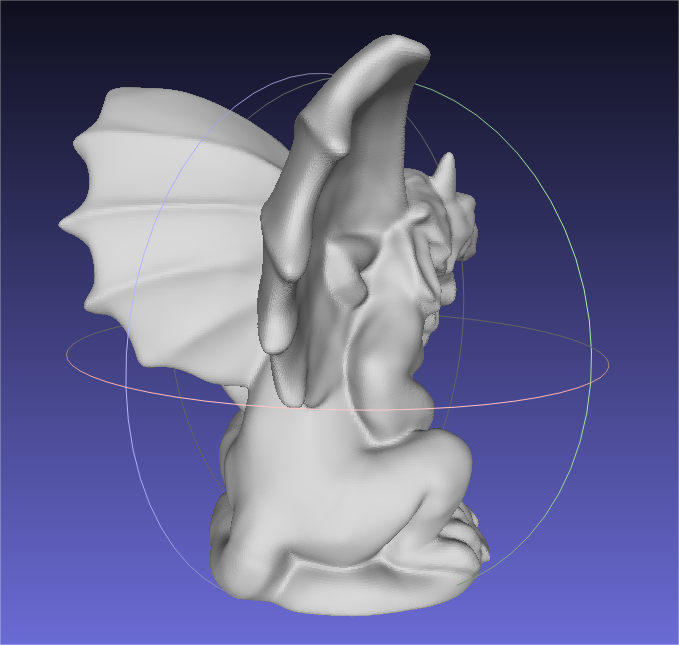
\includegraphics[width=0.9\linewidth]{figures/4.png}
    \end{subfigure}
    \caption{\textbf{Output Mesh}}
\end{figure}


\bibliographystyle{acm}
\nocite{*}
\bibliography{Lab3-report}

\appendix
\section{Appendix}
Requirements: $torch,\ numpy,\ scipy,\ skimage$

Running command: $python\ main.py --args$

$--args$ are given as bellow:

\begin{table}[!htbp]
    \centering
    \begin{tabular}{|c|c|c|c|}
        \hline
        \textbf{Perparameters} & \textbf{Type} & \textbf{Default} & \textbf{Help}                                       \\
        \hline
        $epochs$               & int           & 2400             & Number of trainning epochs                          \\
        \hline
        $resolution$           & int           & 256              & Resolution of output file                           \\
        \hline
        $load$                 & bool          & True             & True: load a model(need cuda); False: train a model \\
        \hline
        $input\_path$          & str           & gargoyle.xyz     & Path of input file                                  \\
        \hline
        $output\_path$         & str           & output.obj       & Path of output file                                 \\
        \hline
        $model\_path$          & str           & model.pt         & Path for load or save model                         \\
        \hline
    \end{tabular}
    \renewcommand{\tablename}{Tab}
    \caption{\textbf{ArgumentParser of main.py}}
\end{table}


\end{document}